\documentclass[12pt,a4paper]{report}

% Essential packages
\usepackage[utf8]{inputenc}
\usepackage{graphicx}
\usepackage{hyperref}
\usepackage{geometry}
\usepackage{xcolor}
\usepackage{titlesec}
\usepackage{float}
\usepackage{listings}
\usepackage{booktabs}
\usepackage{array}
\usepackage{fancyhdr}
\usepackage{enumitem}
\usepackage{parskip}

% Page geometry - reduce margins for more content space
\geometry{
    a4paper,
    top=2cm,
    bottom=2cm,
    left=2cm,
    right=2cm,
    headheight=14pt,
    includehead
}

% Colors
\definecolor{linkcolor}{RGB}{0,83,155}
\definecolor{codegreen}{rgb}{0,0.6,0}
\definecolor{codegray}{rgb}{0.5,0.5,0.5}
\definecolor{codepurple}{rgb}{0.58,0,0.82}
\definecolor{backcolour}{rgb}{0.95,0.95,0.92}

% Hyperref setup
\hypersetup{
    colorlinks=true,
    linkcolor=linkcolor,
    filecolor=linkcolor,
    urlcolor=linkcolor,
}

% Title formatting - reduce spacing
\titleformat{\chapter}{\normalfont\LARGE\bfseries}{\thechapter.}{1em}{}
\titlespacing*{\chapter}{0pt}{0pt}{10pt}

\titleformat{\section}{\normalfont\Large\bfseries}{\thesection}{1em}{}
\titlespacing*{\section}{0pt}{10pt}{5pt}

% Adjust spacing for lists - make more compact
\setlist{noitemsep,topsep=0pt,parsep=0pt,partopsep=0pt,leftmargin=*}
\setlist[itemize]{label=\textbullet}

% Listing style - optimize space
\lstdefinestyle{mystyle}{
    backgroundcolor=\color{backcolour},   
    commentstyle=\color{codegreen},
    keywordstyle=\color{magenta},
    stringstyle=\color{codepurple},
    basicstyle=\ttfamily\small,
    breakatwhitespace=false,         
    breaklines=true,                 
    captionpos=b,                    
    keepspaces=true,                 
    numbers=left,                    
    numbersep=5pt,                  
    showspaces=false,                
    showstringspaces=false,
    showtabs=false,                  
    tabsize=2,
    frame=single,
    framesep=3pt,
    framexleftmargin=5pt,
    xleftmargin=15pt,
    belowskip=0.5\baselineskip,
    aboveskip=0.5\baselineskip
}
\lstset{style=mystyle}

% Header and footer
\pagestyle{fancy}
\fancyhf{}
\rhead{\thepage}
\lhead{Intelligent Open Source License Recommendation System}
\renewcommand{\headrulewidth}{0.4pt}

% Make chapter pages also use fancy style
\makeatletter
\renewcommand{\chapter}{\if@openright\cleardoublepage\else\clearpage\fi
  \thispagestyle{fancy}%
  \global\@topnum\z@
  \@afterindentfalse
  \secdef\@chapter\@schapter}
\makeatother

% Optimize paragraph spacing
\setlength{\parindent}{0pt}
\setlength{\parskip}{3pt}  % Reduced from 6pt

% Table spacing
\renewcommand{\arraystretch}{1.2}

% Figure spacing
\setlength{\floatsep}{10pt}
\setlength{\textfloatsep}{10pt}
\setlength{\intextsep}{10pt}

% Table of contents spacing
\setcounter{tocdepth}{2}
\renewcommand{\baselinestretch}{1.1}

\begin{document}

% Cover page
\begin{titlepage}
    \centering
    \vspace*{-1cm}
    % Nankai University Logo
    
\includegraphics[width=0.4\textwidth]{nankai-logo.pdf}\\[1cm]
    {\large\bfseries Nankai University\\[1cm]}

    {\Huge\bfseries Intelligent Open Source License\\Recommendation System\\[1cm]}

    {\Large\bfseries Technical Report\\[0.5cm]}

    {\large\bfseries A Modern Approach to License Selection}\\[1.5cm]

    {\largeb\bfseries Prepared by:\\[0.5cm]
    \begin{tabular}{ll}
        Name               & Student ID \\
        \hline
        Zamo Rzgar Ahmed   & 2120246004 \\
        Naser Al Musalhi   & 2120246005 \\
        Gheith Alrawahi    & 2120246006 \\
        Gheyath AL Mamoori & 2120246020 \\
        Mohamed Sidi       & 2120246048 \\
    \end{tabular}\\}

\end{titlepage}

% Table of contents
\pagestyle{fancy}
\tableofcontents
\thispagestyle{fancy}

% Force fancy style for the first page after TOC
\clearpage
\thispagestyle{fancy}

% Introduction
\chapter{Introduction}
In the modern era of collaborative software development, open source licenses serve as vital instruments that define the terms under which software can be used, modified, and distributed. Licenses ensure legal protection, promote transparency, and foster community trust. Despite their importance, many developers, especially those new to open source, struggle to choose a license that aligns with their values and project goals.

This project was created to simplify the license selection process for open source developers. It allows users to answer a few structured questions, then automatically suggests the most suitable license based on their answers. This reduces confusion, saves time, and ensures legal clarity for developers and users alike.

% Installation Guide
\chapter{Installation Guide}
This section provides step-by-step instructions for setting up the project locally.

\section{Prerequisites}
Before installing the project, ensure you have the following prerequisites installed:
\begin{itemize}
    \item PHP 8.2 or higher
    \item Composer (PHP package manager)
    \item Node.js and npm
    \item Git
\end{itemize}

\section{Installation Steps}
Follow these steps to set up the project:

\begin{enumerate}[label=\arabic*.]
    \item Clone the repository:
          \begin{lstlisting}[language=bash]
git clone https://github.com/gheith3/open-license-generator.git
cd open-license-generator
    \end{lstlisting}

    \item Install PHP dependencies:
          \begin{lstlisting}[language=bash]
composer install
    \end{lstlisting}

    \item Create environment file:
          \begin{lstlisting}[language=bash]
cp .env.example .env
php artisan key:generate
    \end{lstlisting}

    \item Configure the database in .env file:
          \begin{lstlisting}
DB_CONNECTION=sqlite
DB_DATABASE=/absolute/path/to/database.sqlite
    \end{lstlisting}

    \item Create the SQLite database:
          \begin{lstlisting}[language=bash]
touch database/database.sqlite
php artisan migrate
    \end{lstlisting}

    \item Seed the database with initial data:
          \begin{lstlisting}[language=bash]
php artisan db:seed
    \end{lstlisting}

    \item Install frontend dependencies:
          \begin{lstlisting}[language=bash]
npm install
npm run dev
    \end{lstlisting}

    \item Start the development server:
          \begin{lstlisting}[language=bash]
php artisan serve
    \end{lstlisting}
\end{enumerate}

After completing these steps, you can access the application at \texttt{http://localhost:8000}.

% Project Objectives
\chapter{Project Objectives}
\begin{itemize}
    \item To simplify open source license selection through guided user input.
    \item To educate users on key licensing concerns (e.g., attribution, commercial use).
    \item To enable extensibility through a dynamic, database-driven architecture.
    \item To build the application entirely with open source tools and technologies.
\end{itemize}

% System Architecture
\chapter{System Architecture}
\section{Technologies Used}
This application is developed using a modern open source stack:
\begin{itemize}
    \item \textbf{Laravel 12}: Web framework for backend and routing.
    \item \textbf{Livewire}: Enables dynamic and reactive components.
    \item \textbf{Filament}: Admin panel and UI builder for Laravel.
    \item \textbf{SQLite}: Lightweight database for simplicity and portability.
    \item \textbf{PHP 8.2} and \textbf{Composer}: Programming language and dependency manager.
    \item \textbf{PHPUnit}: Automated testing framework.
\end{itemize}

\section{Database Design}
\begin{itemize}
    \item \texttt{LicenseTemplate}: Stores metadata and full text of licenses.
    \item \texttt{Question}: Stores each decision-making prompt.
    \item \texttt{Option}: Possible answers to each question.
    \item \texttt{OptionLicenseScore}: Scores linking options to license recommendations.
    \item \texttt{GeneratedLicense}: User-specific license results.
\end{itemize}

% Methodology
\chapter{Methodology}
\section{Question Design}
The system uses a small set of high-impact questions to evaluate user intent. Each question corresponds to a major licensing principle:

\begin{enumerate}
    \item Should the software be usable with minimal restrictions?
    \item Should derivative works be open sourced?
    \item Should users give credit to the original author?
    \item Should commercial use be allowed?
\end{enumerate}

Each option (typically "Yes" or "No") is scored for every license template. This score reflects how well the option aligns with the goals of that license.

\section{Scoring Algorithm}
The system uses a weighted scoring system:

\begin{table}[h]
    \centering
    \begin{tabular}{lccc}
        \toprule
        Question                    & MIT & GPL & Apache \\
        \midrule
        Minimal restrictions        & 3   & 1   & 2      \\
        Open source for derivatives & 1   & 3   & 2      \\
        Attribution required        & 2   & 3   & 2      \\
        Allow commercial use        & 3   & 1   & 3      \\
        \bottomrule
    \end{tabular}
    \caption{License Scoring Matrix}
\end{table}

\section{System Flexibility and Extensibility}
A unique feature of this system is its fully dynamic design. The system allows easy addition of new licenses and questions without modifying code:

\begin{itemize}
    \item New licenses are added via the \texttt{LicenseTemplate} table.
    \item New questions and answer options are added via the \texttt{Question} and \texttt{Option} models.
    \item \texttt{OptionLicenseScore} links every answer to a license score.
\end{itemize}

% Results and Screenshots
\chapter{Results and Screenshots}
\section{System Interface}
\begin{figure}[H]
    \centering
    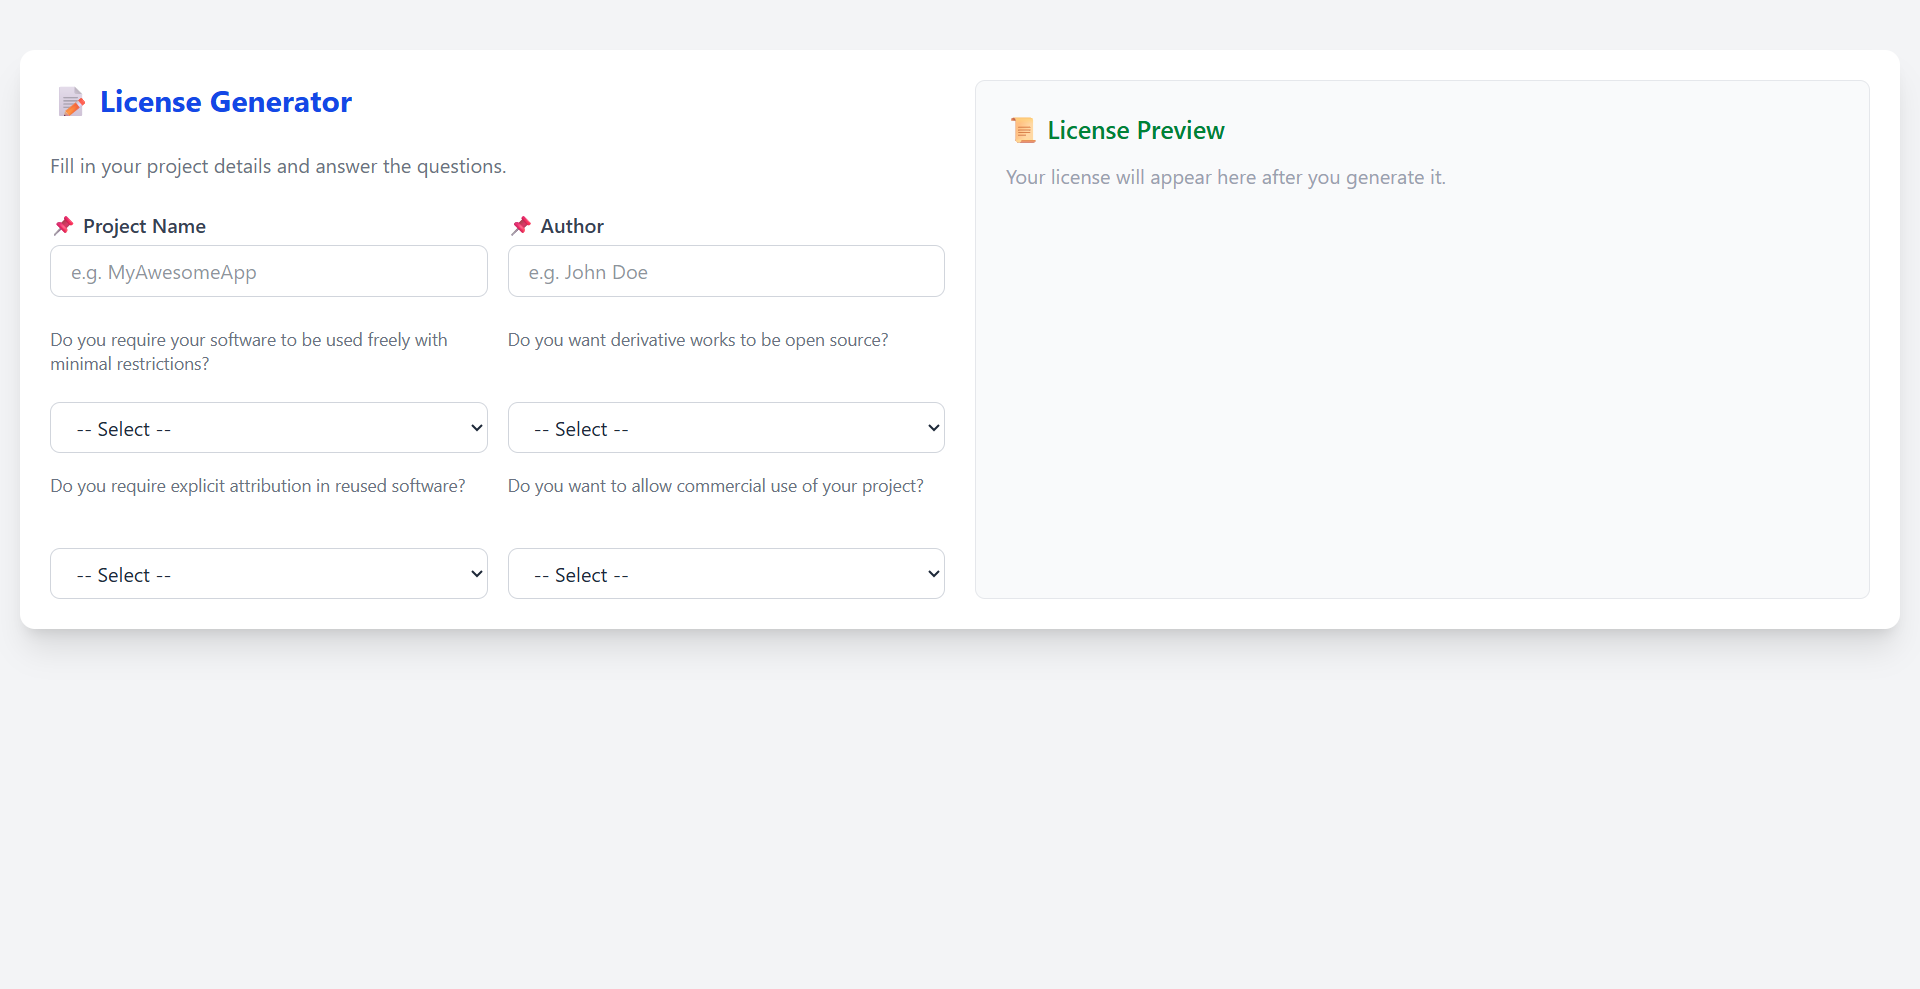
\includegraphics[width=0.9\textwidth]{Screenshots/os0.png}
    \caption{Index Page}
\end{figure}

\begin{figure}[H]
    \centering
    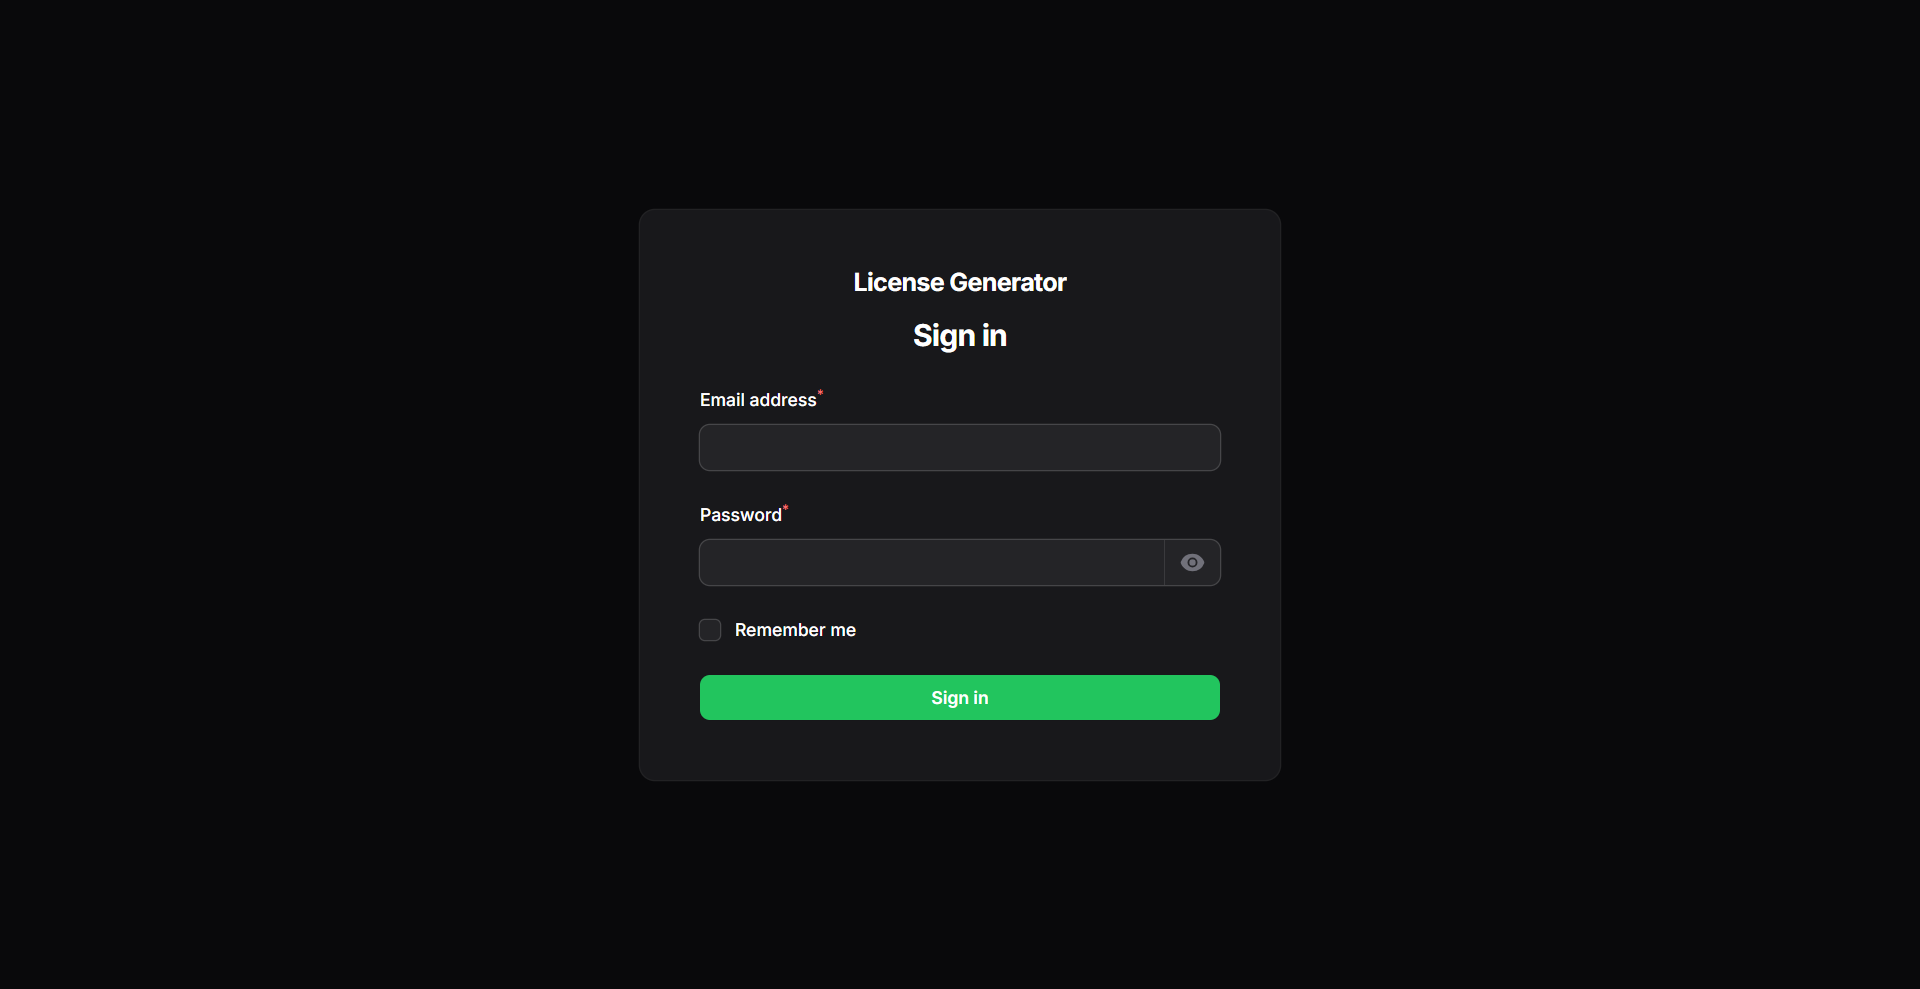
\includegraphics[width=0.9\textwidth]{Screenshots/os3.png}
    \caption{Admin Panel Signin}
\end{figure}

\begin{figure}[H]
    \centering
    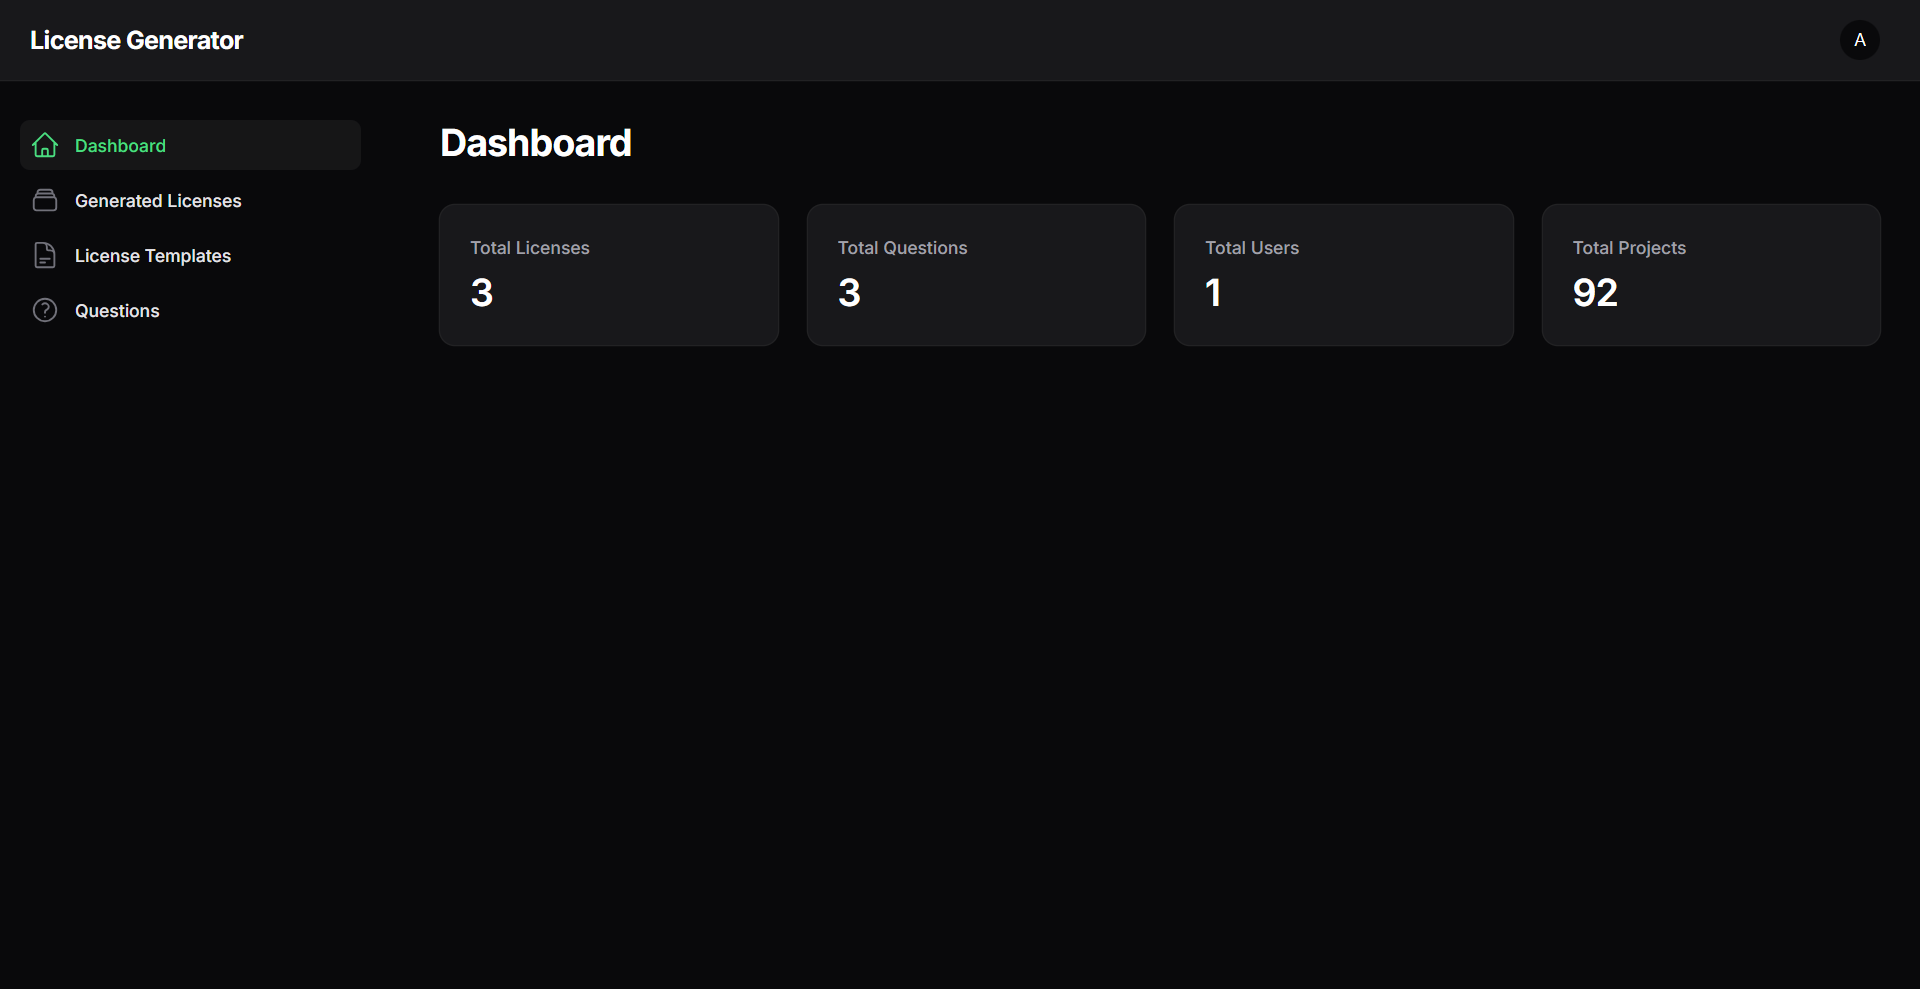
\includegraphics[width=0.9\textwidth]{Screenshots/os4.png}
    \caption{Admin Dashboard}
\end{figure}

\begin{figure}[H]
    \centering
    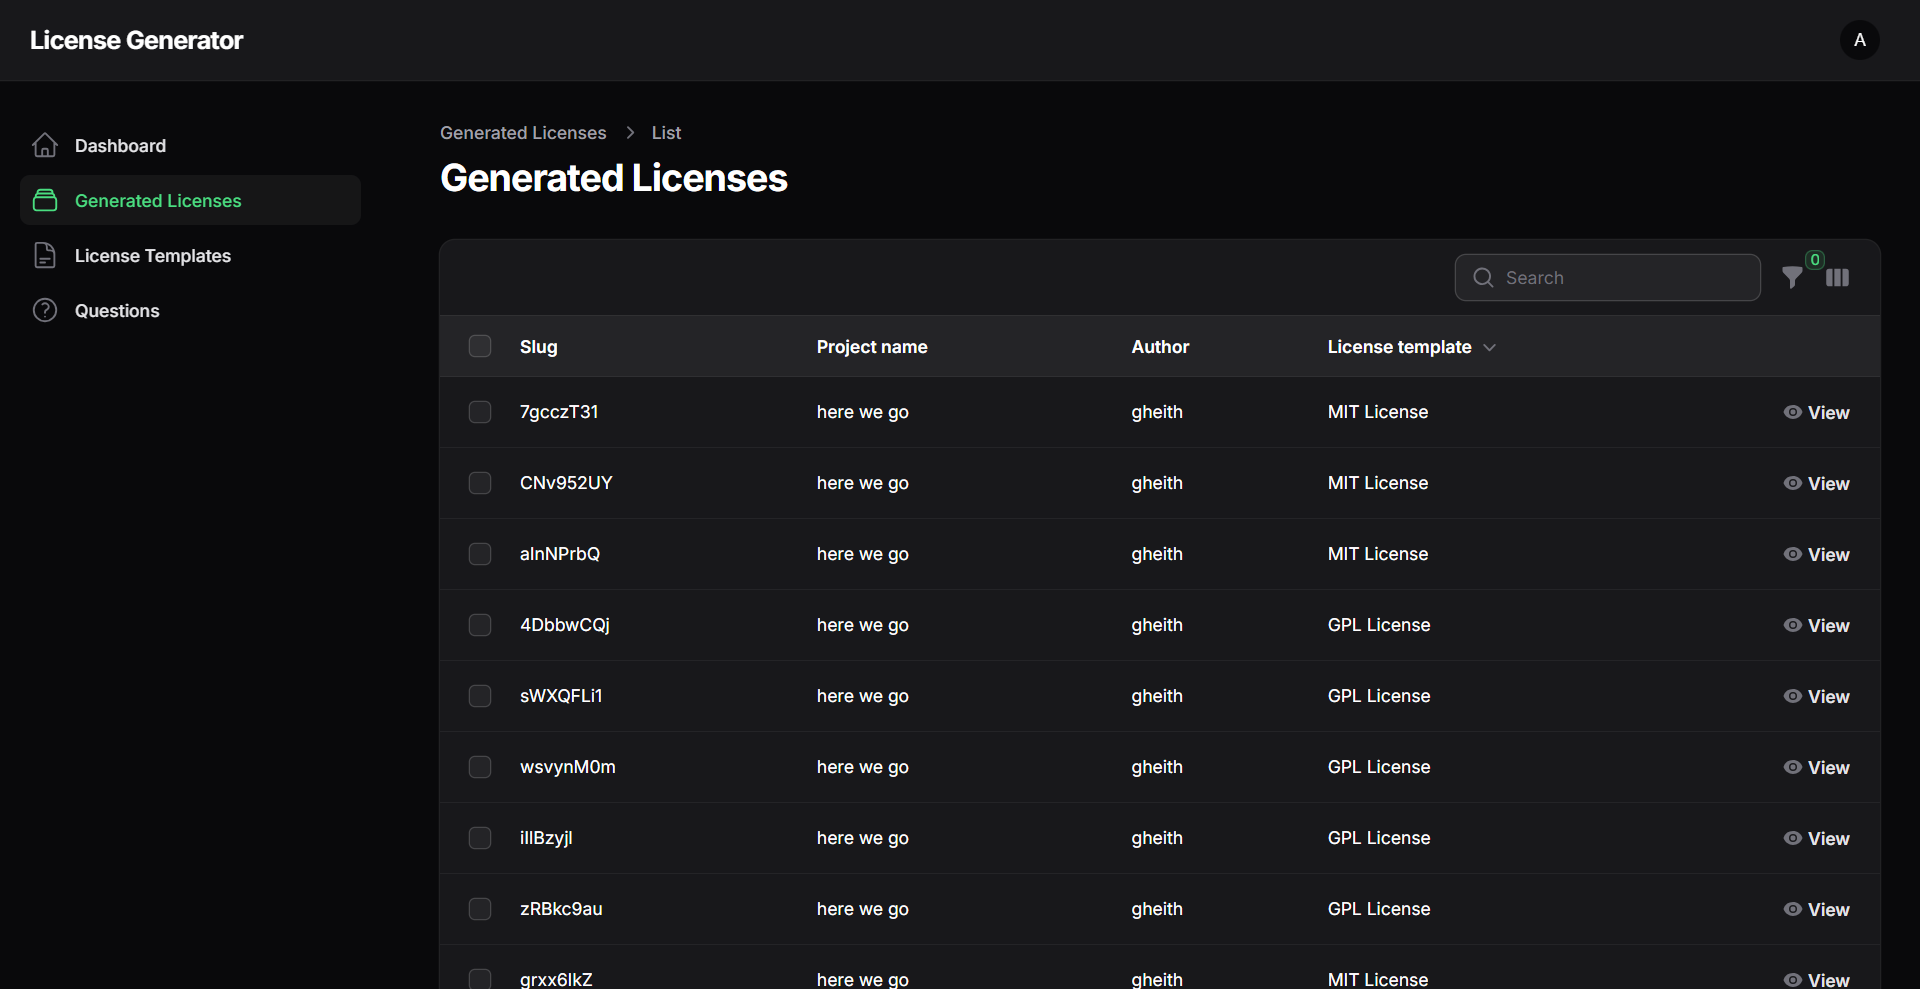
\includegraphics[width=0.9\textwidth]{Screenshots/os5.png}
    \caption{License Management}
\end{figure}

\begin{figure}[H]
    \centering
    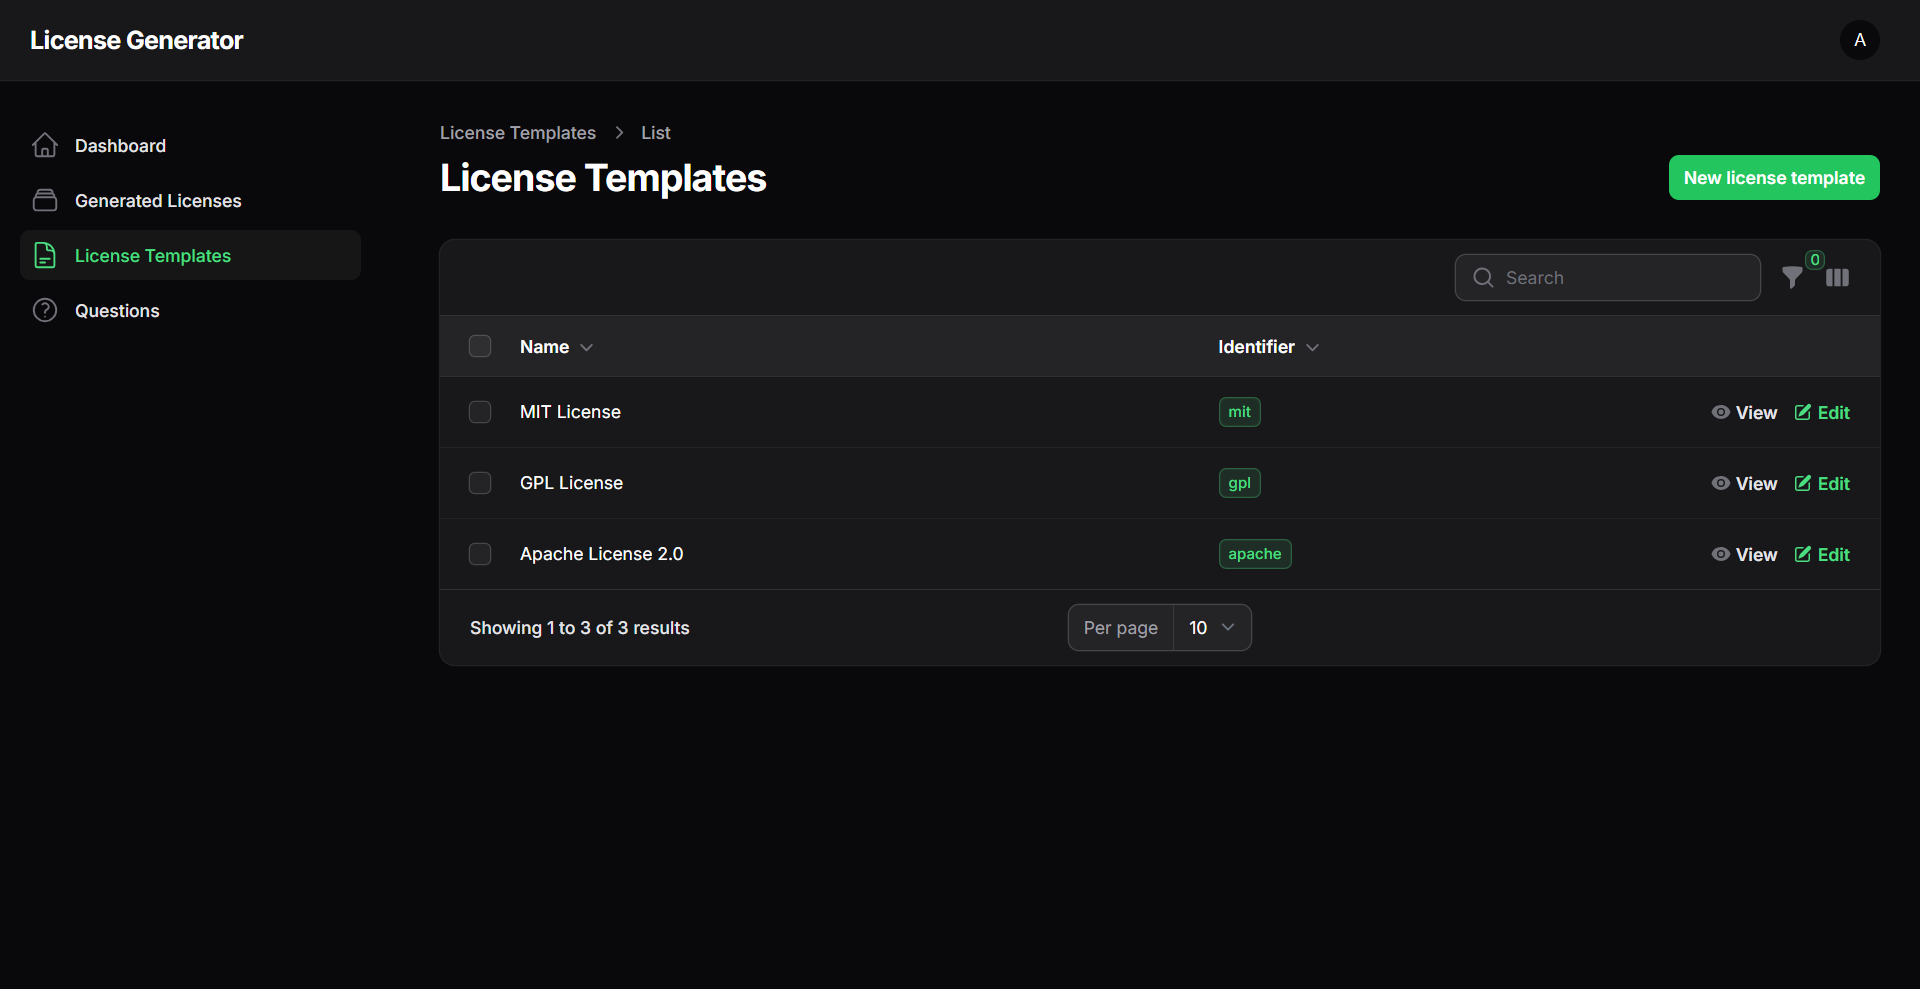
\includegraphics[width=0.9\textwidth]{Screenshots/os6.png}
    \caption{Question Management}
\end{figure}

\begin{figure}[H]
    \centering
    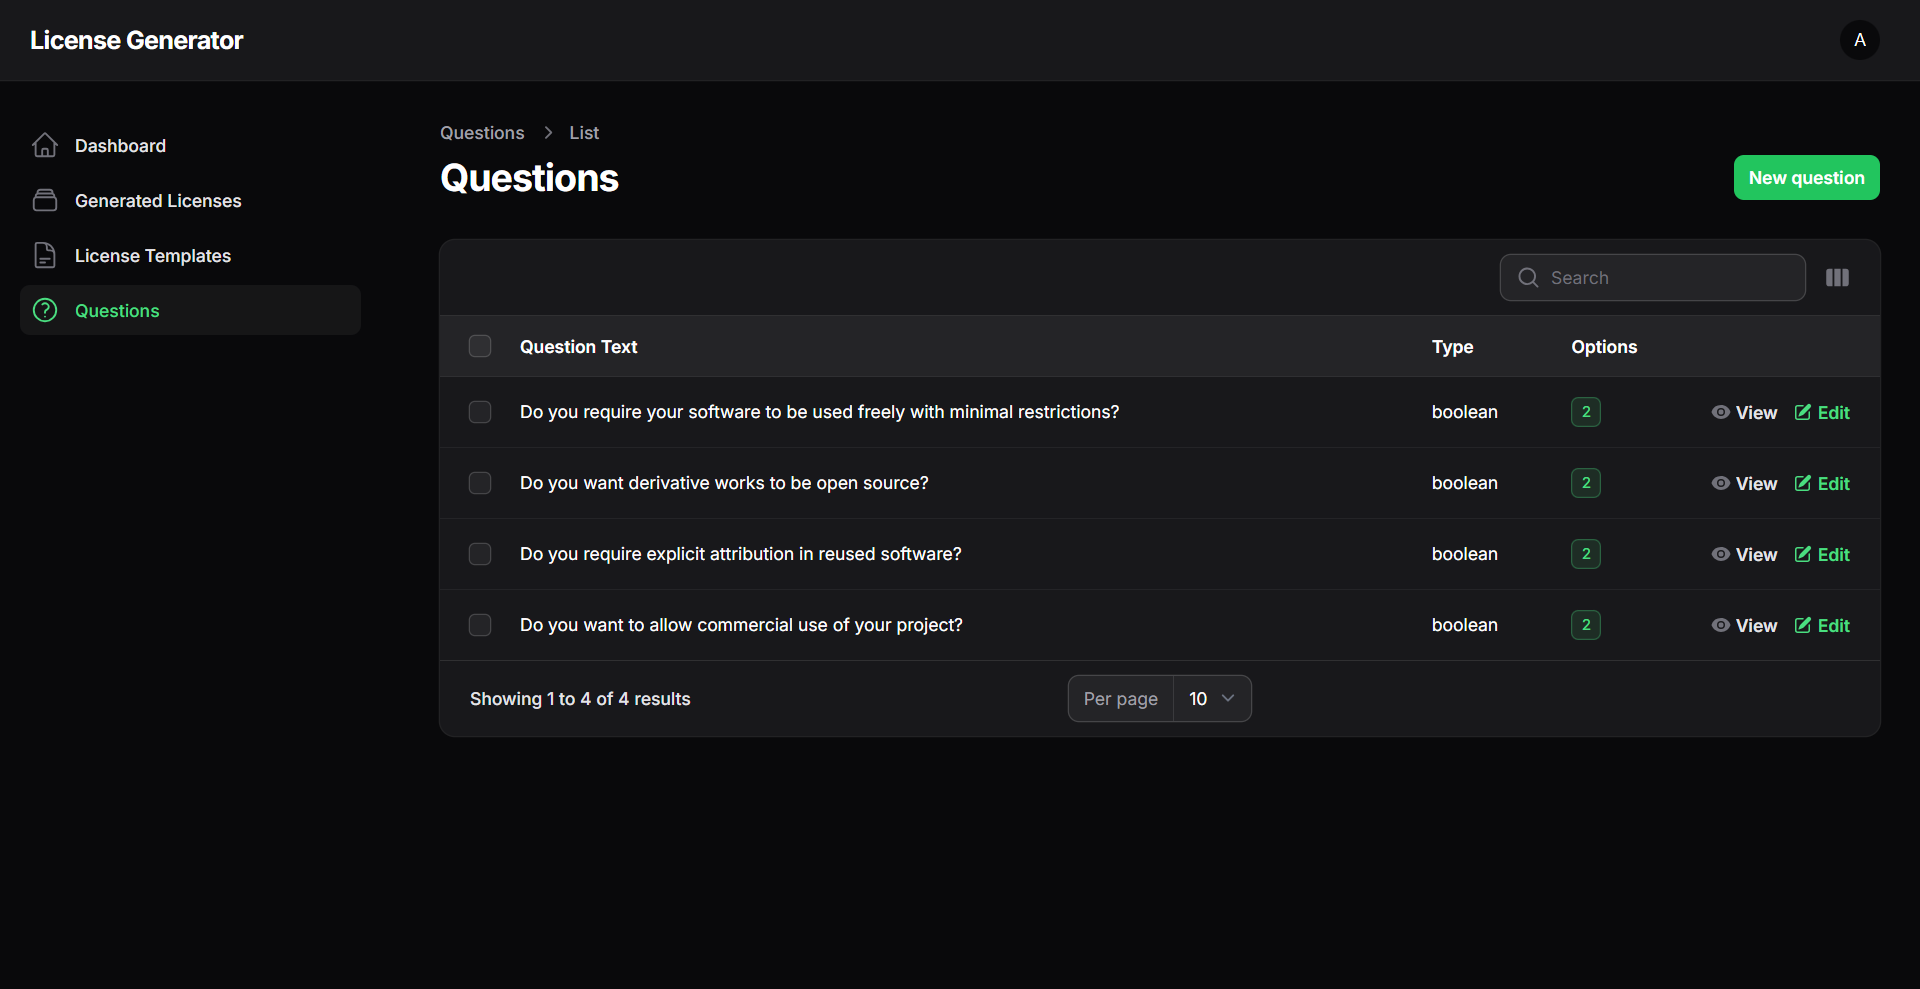
\includegraphics[width=0.9\textwidth]{Screenshots/os7.png}
    \caption{User Interface}
\end{figure}

\begin{figure}[H]
    \centering
    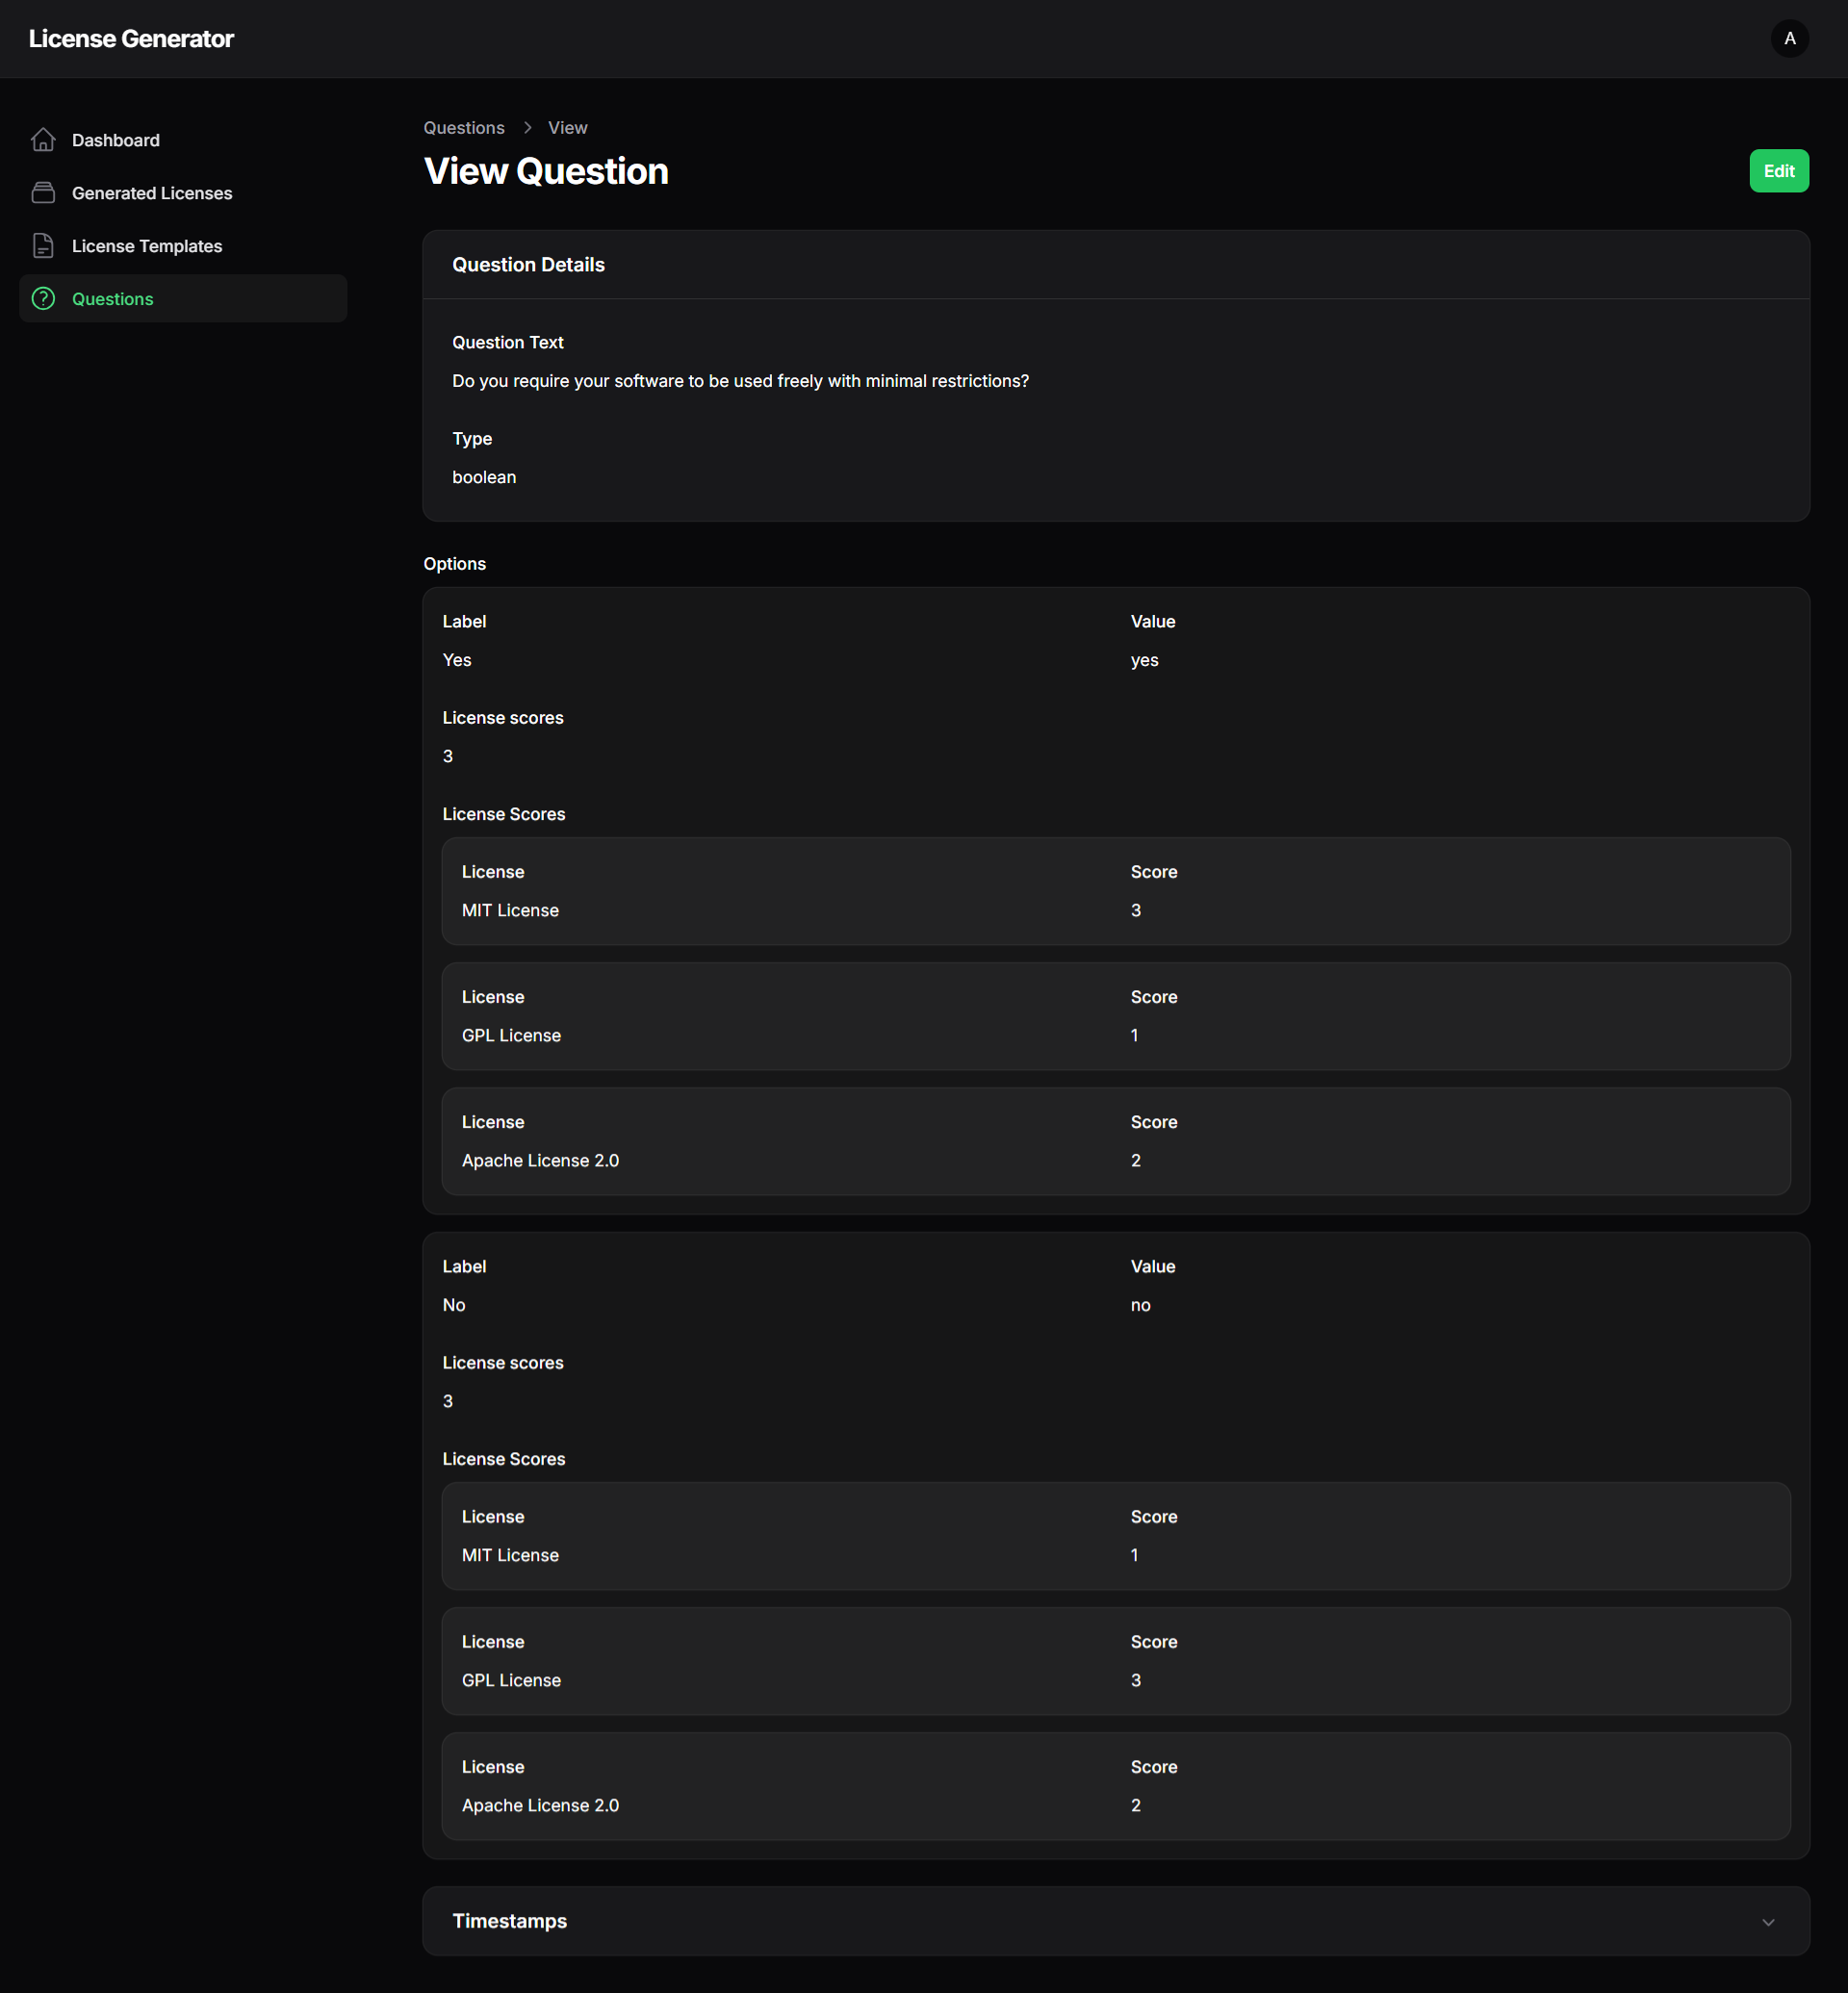
\includegraphics[width=0.9\textwidth]{Screenshots/os8.png}
    \caption{Results Display}
\end{figure}

\begin{figure}[H]
    \centering
    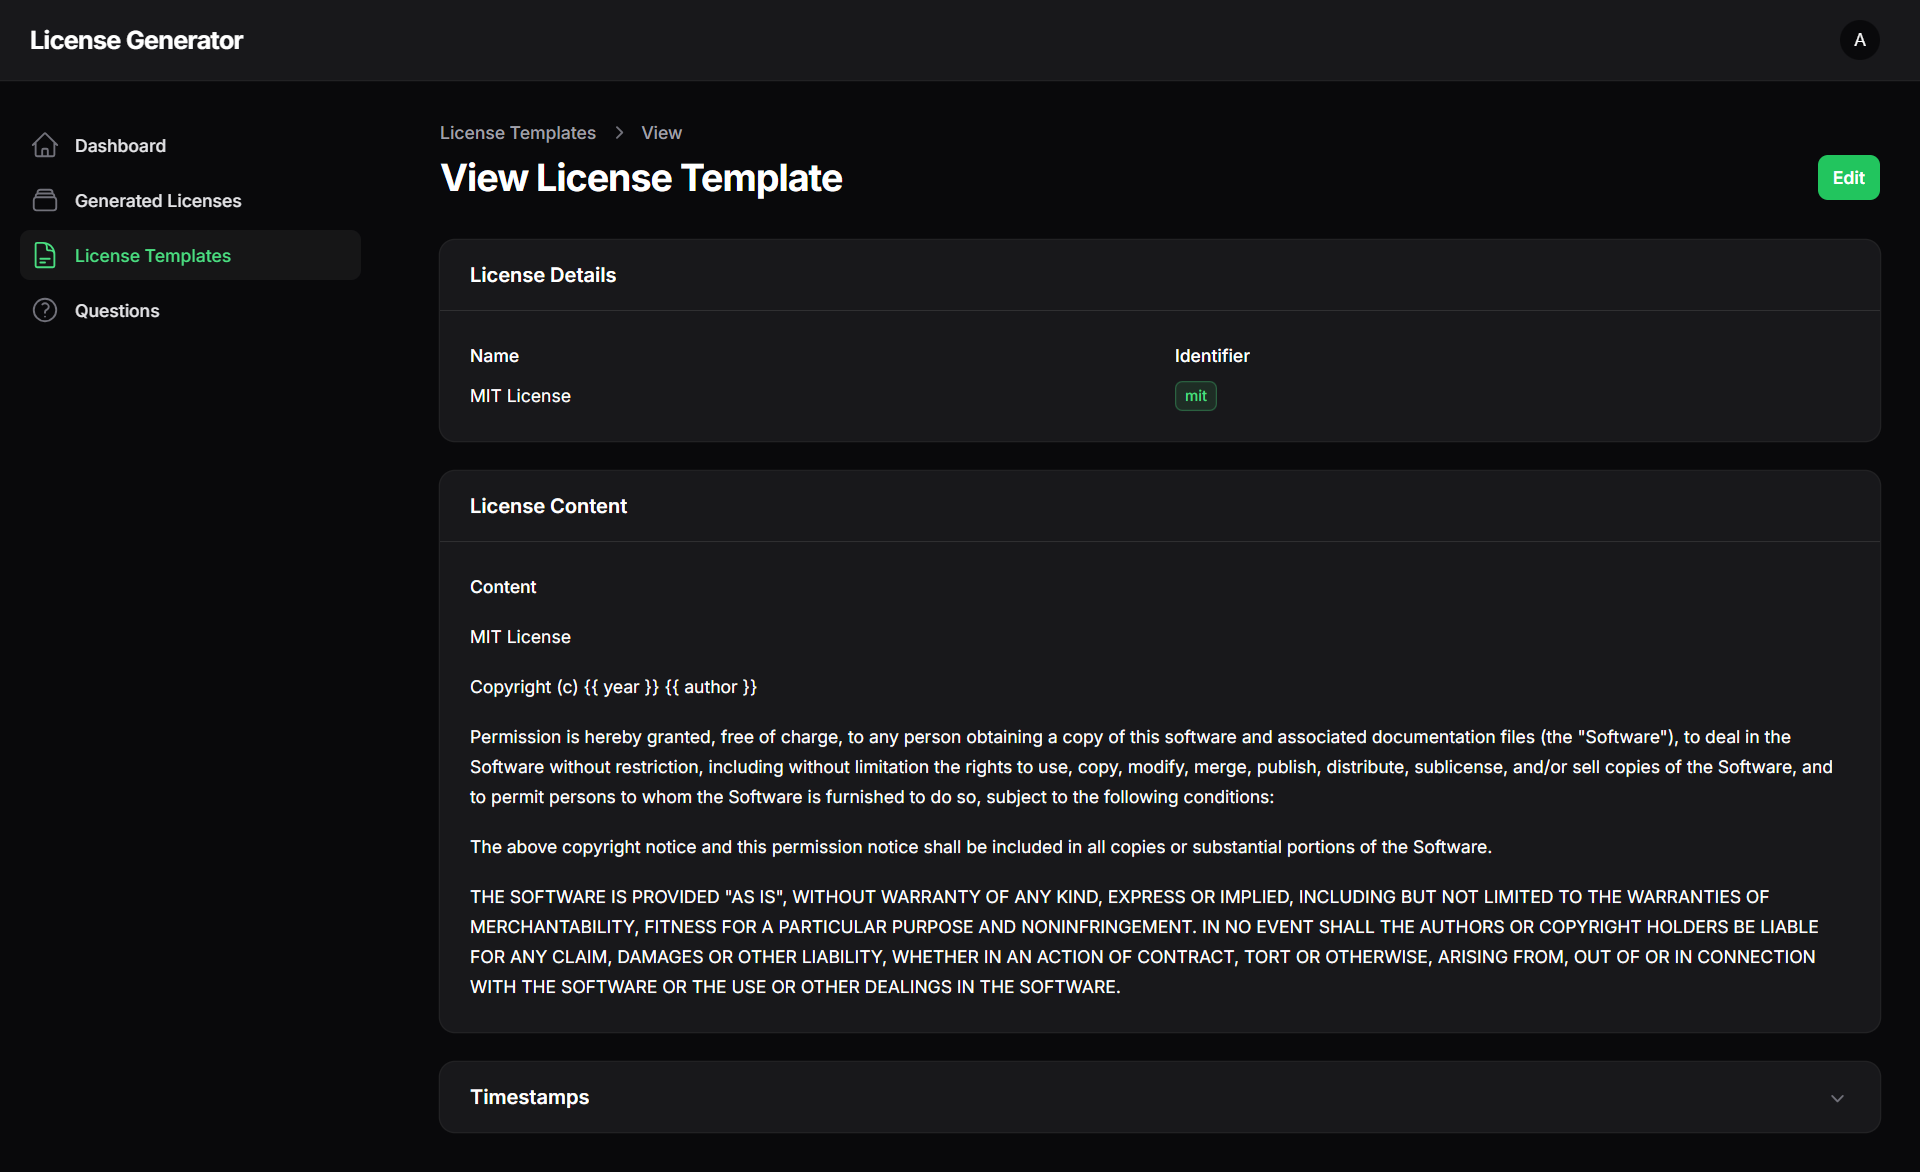
\includegraphics[width=0.9\textwidth]{Screenshots/os9.png}
    \caption{System Overview}
\end{figure}

% Conclusion
\chapter{Conclusion}
The Intelligent Open Source License Recommendation System is an effective and extensible tool designed to help developers make informed licensing decisions. Built entirely with open technologies, it aligns well with the ethos of open source itself. By transforming a complex legal decision into a guided process, the system lowers barriers for developers around the world and promotes sustainable open source practices.

\end{document}